\documentclass[tikz,border=8pt]{standalone}
\usetikzlibrary{automata,positioning,arrows.meta}
\begin{document}
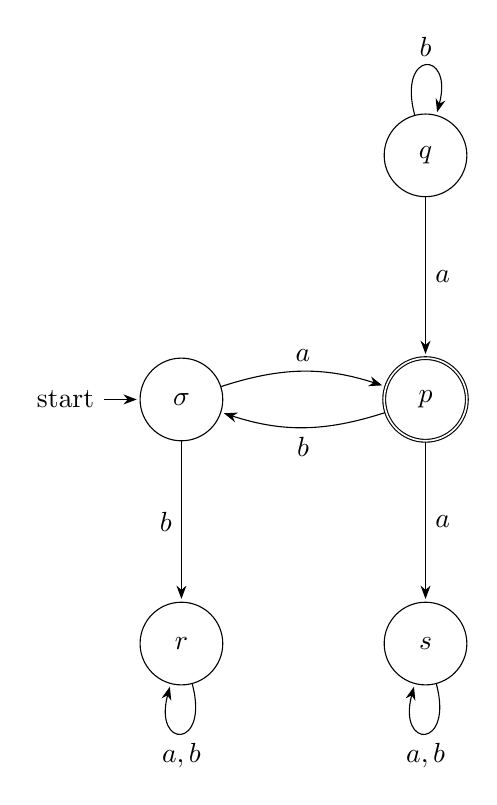
\begin{tikzpicture}[
  >=Stealth,
  shorten >=1pt,
  node distance=3.1cm,
  on grid,
  auto,
  every state/.style={minimum size=1.05cm}
]
  % Reconstructed from the classifications stated in the article:
  % accessible = {sigma,p,r,s}, live = {sigma,p,q}, useful = {sigma,p}.
  \node[state,initial] (sigma) {$\sigma$};
  \node[state,accepting,right=of sigma] (p) {$p$};
  \node[state,below=of sigma] (r) {$r$};
  \node[state,below=of p] (s) {$s$};
  \node[state,above=of p] (q) {$q$};

  \path[->]
    (sigma) edge[bend left=18] node {$a$} (p)
            edge node[left] {$b$} (r)
    (p) edge[bend left=18] node {$b$} (sigma)
        edge node[right] {$a$} (s)
    (q) edge node[right] {$a$} (p)
        edge[loop above] node {$b$} ()
    (r) edge[loop below] node {$a,b$} ()
    (s) edge[loop below] node {$a,b$} ();
\end{tikzpicture}
\end{document}
